\section{Specialization in Scala}
\label{mbox:sec-generics}

\topic{This section presents specialization \cite{iuli-thesis}, a heterogeneous translation for parametric polymorphism in Scala}. Miniboxing builds upon specialization, inheriting its main mechanisms. Therefore a good understanding of specialization and its limitations is necessary to motivate and develop the miniboxing encoding (\S\ref{mbox:sec-miniboxing}) and transformation (\S\ref{mbox:sec-mb-traf}).

\topic{There are two major approaches to translating parametric polymorphism to Java bytecode:} homogeneous, which requires a common representation for all values, and heterogeneous, which duplicates and adapts code for each type. By default, both the Scala and Java compilers use homogeneous translation with each value type having a corresponding reference type. Boxing and unboxing operations jump from one representation to the other. For example, |int| has |java.lang.Integer| as its corresponding reference type.

\topic{Boxing enables a uniform low level data representation, } where all generic type parameters are translated to references. While this simplifies the translation to bytecode, it does come with several disadvantages:
\begin{itemize}
\item Initialization cost: allocating an object, initializing it and returning a pointer takes longer than simply writing to a processor register;
\item Indirect access: Extracting the value from a boxed type requires computing a memory address and accessing it instead of simply reading a processor register;
\item Undermined data locality: Seemingly contiguous memory storages, such as arrays of integers, become arrays of pointers to heap objects, which may not necessarily be aligned in the memory. This can affect cache locality and therefore slow down the execution;
\item Heap cost: the boxed object lives on the heap until it is not referenced anymore and is garbage collected. This puts pressure on the heap and triggers garbage collection more often.
\end{itemize}

\topic{To eliminate the overhead of boxing}, the Scala compiler features specialization: an annotation-driven, compatible and opportunistic heterogeneous transformation. Specialization is based on the premise that not all code is worth duplicating and adapting: code that rarely gets executed or has little interaction with value types is better suited for homogeneous translation. Since a compile-time transformation such as specialization has no means of knowing how code will be used, it relies on programmers to annotate which code to transform. Recent research in JavaScript interpreters \cite{tracemonkey, truffle} uses profiling as another method of triggering compatible specialization of important traces in the program.

\topic{With specialization, programmers explicitly annotate the code} to be transformed heterogeneously (\S\ref{mbox:subsec-spec-class} and \S\ref{mbox:subsec-spec-method}) and the rest of the program undergoes homogeneous translation. The bytecode generated by the two translations is compatible and can be freely mixed. This allows specialization to have an opportunistic nature: it injects specialized code, in the form of specialized class instantiations and specialized method calls (\S\ref{mbox:subsec-spec-rewiring}), but the injected entities are always compatible with the homogeneous translation (\S\ref{mbox:subsec-spec-compatibility}). However, the interaction with separate compilation leads to certain limitations that miniboxing addresses (\S\ref{mbox:subsec-spec-limits}).

\subsection{Class Specialization}
\label{mbox:subsec-spec-class}

To explain how specialization applies the heterogeneous translation, we can use an immutable linked list example:

\begin{lstlisting-nobreak}
 class ListNode[@specialized T]
          (val head: T, val tail: ListNode[T]) {
   def contains(element: T): Boolean = ...
 }
\end{lstlisting-nobreak}

\topic{Each} |ListNode| instance stores an element of type |T| and a reference to the tail of the list. The |null| pointer, placed as the tail of a list, marks its end. A real linked list from the Scala standard library is more sophisticated \cite{collections-alex, adriaan}, but for the purpose of describing specialization this example is sufficient. It is also part of the benchmarks presented in the Evaluation section (\S\ref{mbox:sec-evaluation}), as it depicts the behavior of non-contiguous collections that require random heap access.

\begin{figure}[t!]
    \centering
    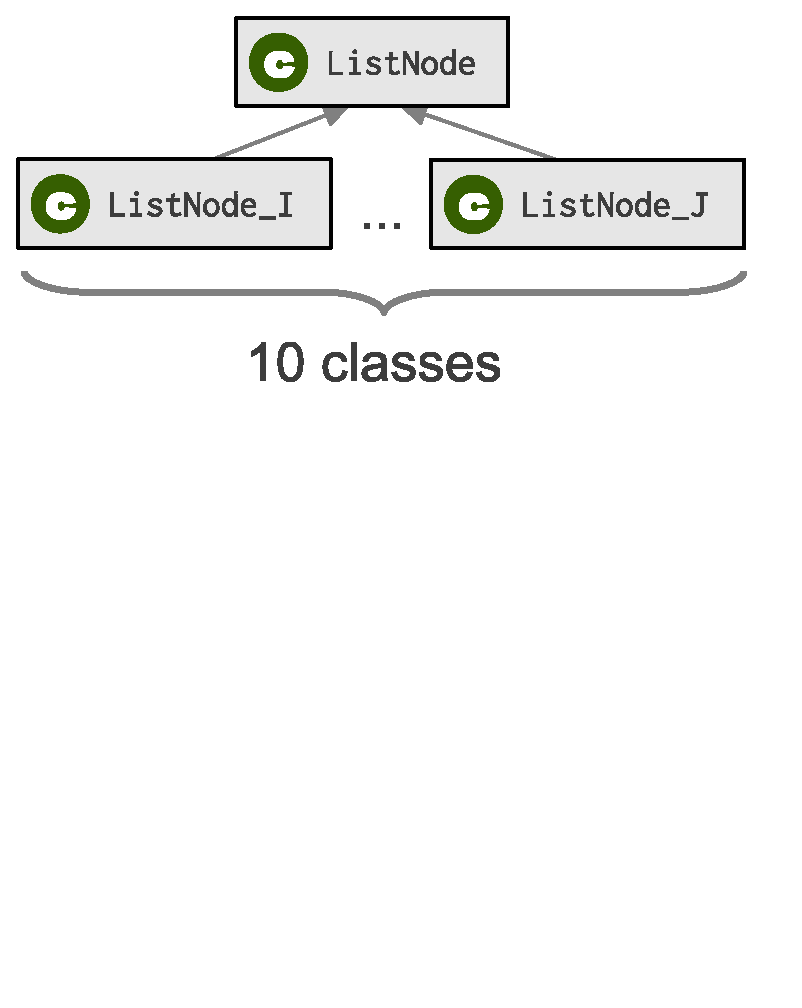
\includegraphics[width=0.5\textwidth]{diags/spec-diag.eps}
    \vspace{-16em}
    \caption{Class hierarchy generated by Specialization. The letters in class suffix represent the type they are specialized for: V-Scala Unit, Z-Boolean, B-Byte \ldots J-Long, L-AnyRef. The names are simplified throughout the chapter, and we avoid discussing the problem of name mangling, which was addressed in \cite{iuli-thesis}.}
    \label{mbox:fig-spec-diag}
\end{figure}

\topic{The} |ListNode| class has the generic |head| field, which needs to be specialized in order to avoid boxing. To this end, specialization will duplicate the class itself and adapt its fields for each primitive value type. Figure \ref{mbox:fig-spec-diag} shows the class hierarchy created: the parent class is the homogeneous translation of |ListNode|, which we also call generic class. The 10 subclasses are the specialized variants. They correspond to the 8 Java primitive types, |Unit| (which is Scala's object-oriented representation of |void|) and reference types\footnote{Technical note: For a single type parameter the reference variant will not be generated and the generic class will be used instead.}. Each of these specialized classes contains a |head| field of a primitive type, and inherits (or overrides) methods defined in the generic class. So far, specialization duplicated the class and adapted the fields, but in order to remove boxing the methods also need to be transformed heterogeneously.

\subsection{Method Specialization}
\label{mbox:subsec-spec-method}

\topic{In the specialized variants of} |ListNode|, the |contains| method needs to be duplicated and adapted to accept primitive values as arguments instead of their boxed representations. Since the |contains| method is already inherited from the generic class, it actually needs to be overridden. But it cannot be overridden, because its signature after the erasure \cite{java-erasure} transformation expects a reference type (|java.lang.Object|) and the specialized signature expects a primitive value. Therefore specialized methods need to be name-mangled, giving birth to new methods such as |contains_I| for |Int| and |contains_J| for |Long|.

\begin{figure}[t!]
    \vspace{-0.5em}
    \centering
    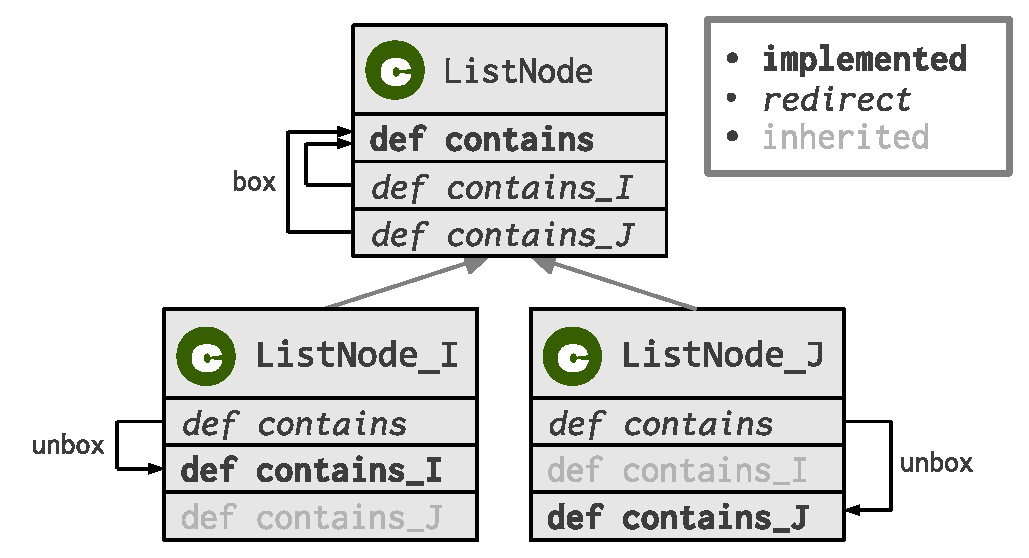
\includegraphics[width=0.65\textwidth]{diags/spec-methods.eps}
    \caption{Method overriding and redirection for ListNode and two of its specialized variants. Constructors and accessors are omitted from this diagram.}
    \label{mbox:fig-redirects}
    \vspace{-0.5em}
\end{figure}

\topic{The} |contains| method from the generic parent class will be inherited by all the specialized classes. But its code is generic and does not make use of primitive values, which is suboptimal. Therefore each specialized class overrides the generic |contains| and redirects it to the corresponding specialized variant, such as |contains_I| or |contains_J|. The redirection is done by unboxing the argument received by |contains| and calling the specialized method with the value type, as shown in Figure \ref{mbox:fig-redirects}. The same transformation is applied for accessors of specialized fields, such as |head| in the |ListNode| class.

\subsection{Opportunistic Tree Transformation}
\label{mbox:subsec-spec-rewiring}

\topic{The program code can only refer to generic classes and methods,} not their specialized variants. This happens because the specialization phase, which creates the variants, runs after the type checking phase. Thus the program is checked only against the generic classes and methods. But this does not mean specialization duplicates code in vain: aside from creating the variants, specialization also injects the specialized variants in the program code.

\topic{The last step in eliminating boxing is rewriting} the Scala abstract syntax tree (AST) to instantiate specialized classes and use specialized methods. We call this process rewiring. Rewiring works across separate compilation, as the specialization metadata is written in the generated bytecode. This makes is possible to use specialized code from libraries.

\topic{The instantiation rewiring injects specialized classes when the \textbf{new} keyword is used}. When the instantiated class has a more specific specialized variant for the given type arguments, the instantiation is rewired. Despite constructing a different class, the types in the AST are not adjusted to reflect this: In the example given below, although the instantiation is rewired to |new ListNode_I|, the type of |node1| remains |ListNode[Int]|. This makes specialization compatible: whether or not the instantiation is rewired, both the specialized class and the generic class are still subtypes of |ListNode[Int]|. Rewiring can only be done if the type arguments are statically known:

\begin{lstlisting-nobreak}
 // before rewiring:
 val node1: ListNode[Int] =
        new ListNode[Int](3, null)
 // after rewiring:
 val node1: ListNode[Int] =
        new ListNode_I(3, null)
 // not rewired if U is an abstract type or the
 // type parameter of an enclosing class/method
 val node2: ListNode[U] =
        new ListNode[U](u, null)
\end{lstlisting-nobreak}

\topic{The next step of rewiring changes inheritance relations} when parent classes have specialized variants that match the type arguments. This injects specialized variants of a class in the inheritance chain, making it possible to use unboxed values when extending a specialized class. This is yet another opportunistic transformation, since the inheritance relation is only rewritten if the type arguments are known statically, as shown by the following example:
%This is another opportunistic transformation, since the inheritance relation is only rewritten if the type parameter is known statically:

\begin{lstlisting-nobreak}
 // before rewiring:
 class IntNode(head: Int, tail: IntNode)
         extends ListNode[Int](head, tail)
 // after rewiring:
 class IntNode(head: Int, tail: IntNode)
         extends ListNode_I(head, tail)
 // not rewired, T not known statically:
 class MyNode[T](head: T, tail: MyNode[T])
         extends ListNode[T](head, tail)
\end{lstlisting-nobreak}

\topic{The two rewirings above inject specialized classes in the code.} Still, call sites point to the homogeneous methods, which use boxed values. The last rewiring addresses methods, which are rewritten depending on the type of their receiver. Any call site with a specialization-annotated receiver for which the type argument is statically known is rewritten to use specialized versions of the methods. In the first call site of the example below, the receiver is the specialization-annotated class |ListNode| and the type argument is statically known to be |Int|. Therefore the call to |contains| is rewired to the specialized |contains_I|:

\begin{lstlisting-nobreak}
 // before rewiring:
 (node1: ListNode[Int]).contains(3)
 // after rewiring:
 (node1: ListNode[Int]).contains_I(3)
 // not rewired if U is an abstract type or the
 // type parameter of an enclosing class/method
 (node2: ListNode[U]).contains(u)
\end{lstlisting-nobreak}

\subsection{Specialization Compatibility}
\label{mbox:subsec-spec-compatibility}

\topic{Since the rewiring process only takes place for statically known type arguments,} the generic class and its specialized subclasses may be mixed together. In the following snippet, the first branch of the |if| statement is rewired to create an instance of |ListNode_I| while the second branch calls the |node| method, whose type parameter |T| is not annotated for specialization, and thus creates the generic class |ListNode|. Therefore, the value |lst| (of static type |ListNode[Int]|) may be either an instance of |ListNode_I| or of |ListNode|, depending on the random condition:

\begin{lstlisting-nobreak}
 // new ListNode[T] not rewired to
 // ListNode_I since T is a type parameter
 def node[T](t: T) = new ListNode[T](t, null)

 val lst: ListNode[Int] =
   if (Random.nextInt().isEven)
     new ListNode[Int](1, null) // ListNode_I
   else
     node(2)                             // ListNode

 lst.contains(0) // rewired to contains_I
\end{lstlisting-nobreak}

\topic{Therefore,} calling a specialized method, |contains_I| in this case, can have as receivers both the generic class, |ListNode|, and the specialized one, |ListNode_I|. So both classes must implement the specialized method. To do so, in |ListNode|, |contains| will be implemented using generic code and |contains_I| will box the argument and call |contains|. In |ListNode_I|, |contains_I| will be implemented using primitive value types and |contains| will unbox and redirect. This can be generalized to multiple specialized variants, as can be seen in Figure \ref{mbox:fig-redirects}: The generic class at the top of the hierarchy contains all specialized variants of the |contains| method as redirects to the generic method. Then, each specialized variant of the class inherits from the generic class and overrides its corresponding specialized methods (such as |contains_I| for |ListNode_I|) with the heterogeneously transformed code and redirects the generic method to the specialized variant.

\topic{This shows the compatible nature of specialization:} in order to avoid boxing, both the call site and the receiver need to be rewired, which means the receiver needs to be specialized and the call site needs to know the type arguments statically or be part of code that will be specialized. But if either condition is not fulfilled, the code remains compatible by boxing, either at the call site itself or inside the redirecting method.

\topic{From the perspective of typing the abstract syntax trees}, compatibility is achieved because types are assigned before the specialization phase and are not modified later, so they refer to the generic class, even in the presence of rewiring. The first example in \S\ref{mbox:subsec-spec-rewiring} shows that despite rewiring the {\bf new} operator to create an instance of |ListNode_I|, the type of the |node1| value remains |ListNode[Int]|. Thus type-level compatibility is satisfied by |ListNode_I| being a subtype of |ListNode|, and the reverse subtyping is not necessary, as types never refer to |ListNode_I|\footnote{Except for the {\bf this} type and singleton types in the adapted code.}.

\subsection{Limitations of Specialization}
\label{mbox:subsec-spec-limits}

\topic{There are two limitations in specialization:} the bytecode explosion and the crippled specialized class inheritance. We will describe each problem and show how both can be addressed by the miniboxing encoding.

The specialization mechanism for generating variants is static: whenever the compiler encounters a class annotated for specialization, it generates all its variants up front and outputs bytecode for each of them. This is done to support separate compilation.

\topic{Theoretically, the specialized variant creation could be delayed} until the actual usage but this requires that the source files for specialized classes are available in all future compilation stages, exactly like in C++. This approach is undesirable from a user perspective, as it also requires encoding the original compilation flags and state, which can influence the generated code. Therefore the simplest, although bytecode-expensive solution was chosen: to generate specialized variants for all value types during compilation.

\topic{Fulfilling the bytecode compatibility requirements described before,} for $n$ type parameters and full specialization, means the generic class needs to implement $10^n$ methods, of which $10^n - 2$ are then inherited in the specialized subclasses and $2$ are overridden by each of the $10^n$ subclasses. This makes the bytecode size proportional to $10^n$. If the methods were not inherited but defined in each subclass, the bytecode size would be proportional to $10^{2n}$.

\topic{Still, the generic parent design choice affects inheritance between specialized classes.} Figure \ref{mbox:fig-spec-multi} shows an example where the design of specialization bumps into a multiple class inheritance, which is forbidden by Java. In this case, the children inherit from their generic parent, which is suboptimal, since the specialized variants of |MyList| cannot use the specialization in |ListNode|. Experienced Scala programmers might suggest that |MyNode| should be a trait, so it can be mixed in \cite{scalable-component-abstractions}. Indeed this solves the multiple inheritance problem, but creates bytecode proportional to $10^{2n}$, because the compiler desugars the trait into an interface, and each specialized |MyList_*| class has to implement the methods in that interface. Other more technical problems stem from this design choice too, but could be avoided by having an abstract parent class. For example, fields from the generic class are inherited by the specialized classes, therefore increasing their memory footprint. Constructors also require more complex code because instantiating a specialized class calls the constructor of its parent, the generic class, which needs to be prevented from running, such that side effecting operations in the original class' constructor are not executed twice.

\topic{All in all, at the heart of the bytecode explosion problem and thus the other} limitations of specialization, lies the large number of variants per type parameter: 10. For two type parameters, full specialization with correct inheritance creates $10^4$ times the bytecode. In practice this is not acceptable. Therefore a natural question to ask is how can we reduce the number of variants generated per type parameter? This is the question that inspired miniboxing.

